\chapter{Zakończenie}
W poniższym rozdziale omówione zostaną wyniki przeprowadzonych badań. Dokonane zostanie porównanie algorytmu BPA z gotowej biblioteki, autorskiej implementacji algorytmu Delaunay'a oraz gotowych meshy dostępnych w innych pracach naukowych. Ukazane zostaną możliwości poprawy i udoskonalenia programu oraz niedoskonałości, które zostaną naprawione w przyszłości. 

\section{Podsumowanie}
Tematem pracy było zbudowanie skanera 3D oraz wyeksportowanie gotowych modeli do programu Blender. Dane zadanie zostało wykonane pomyślnie. Przeprowadzono analizę dostępnych metod oraz teoretyczną analizę algorytmów. Dokonano szeregu optymalizacji, wpływających na zwiększenie wydajności autorskiego programu. Postawiony problem był złożony, a na ostateczny wygląd modelu wpływał szereg czynników. W poniższej sekcji przytoczone zostaną najważniejsze z nich.
\subsection{Budowa skanera}
W celu odpowiedniej akwizycji danych należało skonstruować skaner 3D. Po wielu testach wyznaczono jego poprawy schemat. Istotnym czynnikiem była platforma poruszająca się ze stałą prędkością kątową. Bez niej zadanie byłoby niemożliwe do zrealizowania. Odpowiedni dobór kamery trójwymiarowej również wywarł wpływ na jakość modeli. W przypadku początkowej kamery Orbbec Astra Mini rozdzielczość zdjęć była niska, wynosiła maksymalnie 640x480 pikseli. Z kolei rozdzielczość Intel RealSense D435i jest prawie dwukrotnie wyższa. Na jakość modelu wpływa jedynie rozdzielczość pionowa kamery. Wynika to ze sposobu w jaki dane są przekształcane. Z każdej klatki brana jest tylko jedna kolumna, więc jej wysokość wpływa na ostateczną gęstość chmury punktów. Im jest ona większa, tym punkty są bliżej siebie, a co za tym idzie ostateczny model staje się dokładniejszy. Kamera podłączona jest do komputera poprzez gniazdo USB 3.2. Spowodowane jest to tym, że waga zapisywanych danych jest bardzo duża. Film trwający 58 sekund, zawierający dane o głębi oraz kolorze obiektu dla rozdzielczości 848x 640, waży około 1.7 GB i 2.3GB dla odpowiednio 15 klatek na sekundę oraz 30 klatek na sekundę. Gniazdko o niższym standardzie nie byłoby w stanie przesłać takiej ilości informacji. Protokół USB 3.2 jest jednak wciąż zbyt niski, by przesyłać nagranie 1280x720 dla 90 klatek. Prawdopodobnie podłączenie kamery bezpośrednio pod złącze PCI-e byłoby w stanie przesłać taki rozmiar danych. Z danych producenta wynika, że dla rozdzielczości 848x480 koloru oraz głębi dla 90 klatek, rozmiar przesyłanych danych to 1172 Mbps.

Kalibracja kamery jest równie ważna co budowa skanera. By otrzymać najlepsze rezultaty należy odpowiednio nastawić moc emitera, ekspozycję oraz odpowiednio skalować dane głębi by pokrywały się one z rzeczywistymi wartościami. Dzięki wykorzystaniu dedykowanego oprogramowania Intel RealSense Viewer oraz Intel RealSense Depth Quality Tool możliwy był podgląd obrazu z kamery w czasie rzeczywistym. Zmniejszyło to czas kalibracji, ponieważ rezultaty były widoczne natychmiast po zatwierdzeniu. Depth Quality Tool pozwala na sprawdzenie, jak wybrane nastawy wpływają na ilość dziur w nagraniu. Im jest ich mniej, tym dane będą mniej przekłamane, a model będzie wierniej oddawał rzeczywisty obiekt.
\subsection{Akwizycja oraz obróbka danych}
Kolejnym istotnym czynnikiem wpływającym na ostateczny wygląd modelu jest wybrana metoda akwizycji danych. W celu implementacji skanera 3D, wybrano metodę triangulacji laserowej. Pozwala ona na uwzględnienie tylko jednej kolumny na raz. Dzięki jej wykorzystaniu przekształcenia trygonometryczne są prostsze w porównaniu do innych metod. Po uzyskaniu danych z kamery RGBD należy je odpowiednio przetworzyć. Bezpośrednie pomiary głębi zawierają przekłamane punkty, które należy odnaleźć. W przeciwnym wypadku wpłyną one na wygląd modelu po triangulacji Delaunay'a, ponieważ zostaną utworzone z nich zbyt duże trójkąty. Często przekłamane punkty mają wartość odpowiadającą maksymalnej rozdzielczości głębi kamery, więc punkty znajdą się wiele metrów dalej niż rzeczywisty model. To znacząco wpływa na pogorszenie jakości gotowego modelu. W celu uniknięcia tych błędów należy odnaleźć przekłamane punkty. W programie dokonano tego przez liczenie średniej odległości punktów od środka układu współrzędnych. Jeśli odległość przekłamanego punktu będzie o wiele większa niż średnia, to zostanie on oznaczony flagą. Oznaczone w ten sposób punkty, poddane zostaną interpolacji w celu wyznaczenia poprawnej ich wartości.
\newline \indent Po przeprowadzeniu testów różnych metod interpolacji, wybrana została interpolacja wielomianem trzeciego stopnia. Uzyskane dzięki niej rezultaty są dobre i wszystkie punkty znajdują się w odpowiednich miejscach. Ich rozłożenie jest bardziej naturalne, niż w przypadku interpolacji liniowej, która bardziej przypominała metodę najbliższych sąsiadów.
\newline \indent Na koniec należało wyznaczyć wysokość skanowanego obiektu. Dzięki temu długość,szerokość i wysokość obiektu były poprawne i można przeprowadzać rzeczywiste pomiary na wirtualnym obiekcie. Możliwe jest zmierzenie pola powierzchni lub objętości tak wytworzonego modelu. Dokonane zostało to poprzez empiryczne wyznaczenie wzoru na wysokość obiektu w zależności od jego pola powierzchni na obrazie oraz odległości od kamery. Podstawiając te dane do wzoru można wyznaczyć rzeczywistą wysokość przedmiotu.
\subsection{Rekonstrukcja powierzchni}
Ostatnim krokiem programu jest rekonstrukcja powierzchni na podstawie chmury punktów. Zaprezentowane zostały wyniki generacji meshu dokonane za pomocą algorytmu BPA. Przedstawiono sposoby optymalizacji oraz implementacji algorytmu Bowyer-Watson, który jest odmianą triangulacji Delaunay'a. W przypadku algorytmu toczącej się kuli dokonano porównania wpływu promienia na ostateczny wygląd obiektu. Z przeprowadzonych badań wynika, że dla wartości R>5$D_{mean}$ generowana siatka zmienia się nieznacznie, przy dużym wzroście czasu obliczeniowego. Analizując wyniki uznano, że warto zacząć poszukiwania promienia od wartości R=3$D_{mean}$. Następnie stopniowo zwiększać jego długość, do momentu kiedy wygląd generowanej siatki przestanie się zmieniać.

W przypadku triangulacji Delaunay'a skupiono się na optymalizacji algorytmu. Jako, że wszystkie punkty z chmury wchodzą w skład ostatecznego obiektu, nie ma żadnych parametrów do ustawienia. Obiekt natomiast można poddać obróbce w programie Blender w celu wygładzenia powstałych ścian oraz odstających wierzchołków. 

\section{Porównanie wyników przeprowadzonych badań }
Poniżej omówione zostaną wyniki przeprowadzonych badań. Przytoczone zostaną modele wygenerowane za pomocą metody triangulacji Delauny'a oraz algorytmu BPA. Zostaną one zestawione z gotowymi modelami dostępnymi w innych pracach naukowych. Omówiona zostanie ich dokładność względem autorskich metod.

Implementacja triangulacji Delaunay'a oraz użycie BPA miały na celu jak najwierniejsze oddanie powierzchni zeskanowanych modeli. Obie te metody nadają się do różnych celów. Triangulacja może być stosowana, gdy nie wszystkie boki obiektu zostały zeskanowane. Kiedy górna warstwa obiektu nie jest widoczna przez kamerę, to powstanie w tym miejscu luka. Takimi obiektami są wszystkie prostopadłościany oraz walce. Natomiast modele dla których uda się utworzyć górną ścianę to na przykład piramida lub stożek. 

Kolejnym istotnym aspektem metody Delaunay'a jest brak dziur w wygenerowanych ścianach. Poprzez połączenie wszystkich punktów trójkątami, nie będzie między nimi prześwitu. Jej ograniczeniem jest długi czas obliczeniowy algorytmu. Nawet po dokonaniu szeregu optymalizacji czas trwania programu jest wciąż wysoki. 
\newline \indent Algorytm BPA również może znaleźć swoje zastosowanie przy generacji tekstur obiektów. Jego zdolność do odwzorowywania kolorów płaszczyzny jest o wiele lepsza niż w przypadku triangulacji. Jego ograniczeniem natomiast są luki w powierzchni. Wynikają one z nierównomiernego rozkładu punktów w chmurze. Część z dziur można poprawić dobierając odpowiednio promień kuli, jednak inne pozostaną. Z przeprowadzonych badań wynika, że w wypadku danego projektu najlepiej wypadł algorytm triangulacji Delaunay'a. Brak luk w gotowym modelu jest ważniejszy, niż dokładna jakość tekstury. 

Do analizy wyników badań przeprowadzonych w projekcie, porównano dokładność odwzorowania powierzchni z gotowymi zdjęciami dostępnymi w innych pracach naukowych. Na rysunku \ref{fig:appleBoxBpa} zostało przedstawione porównanie autorskich modeli jabłka oraz pudełka. Zestawiono je z człowiekiem Armadillo na rysunku \ref{fig:armadillo}. Jest to popularny zbiór danych, służący do testowania algorytmów generacji meshu. Pochodzi on z uczelni Stanford i przez wiele lat służył naukowcom do testowania oraz implementacji nowych metod tworzenia siatki na podstawie chmury punktów. Występuje w publikacjach zarówno o triangulacji Delaunay'a jak i BPA.  

\begin{figure}[H]
\centering
    \begin{minipage}[b]{0.45\linewidth}
        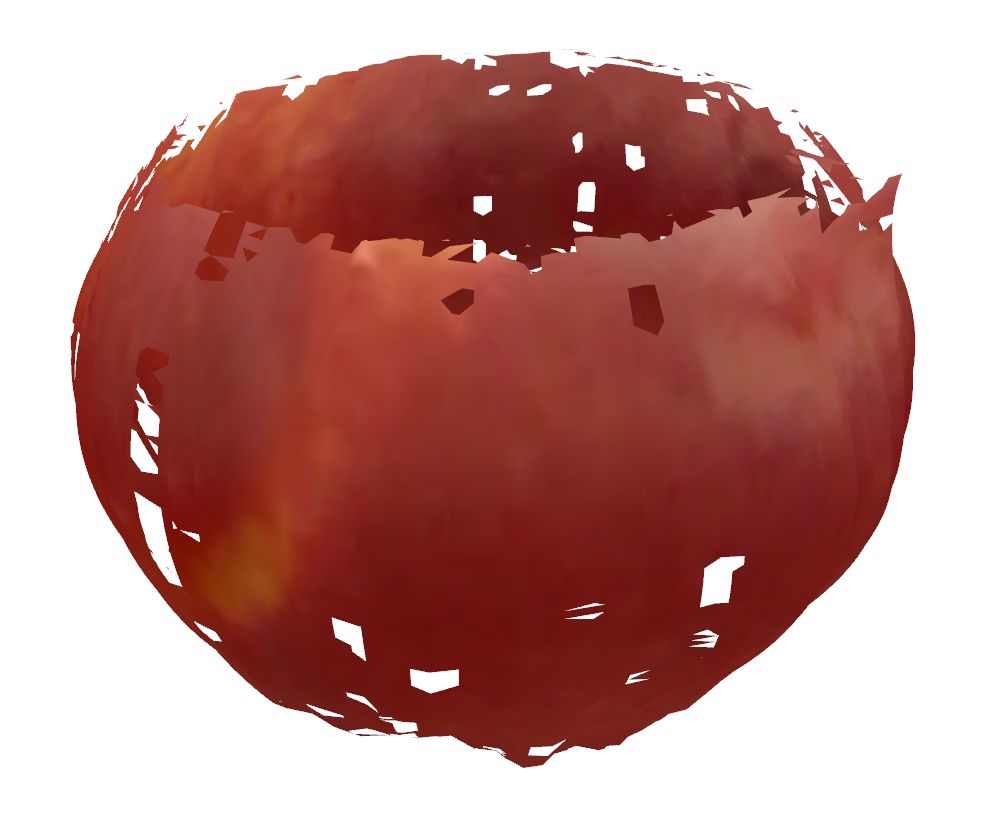
\includegraphics[scale=0.2]{bpaApple7x.PNG}
    \end{minipage}
\quad
    \begin{minipage}[b]{0.45\linewidth}
        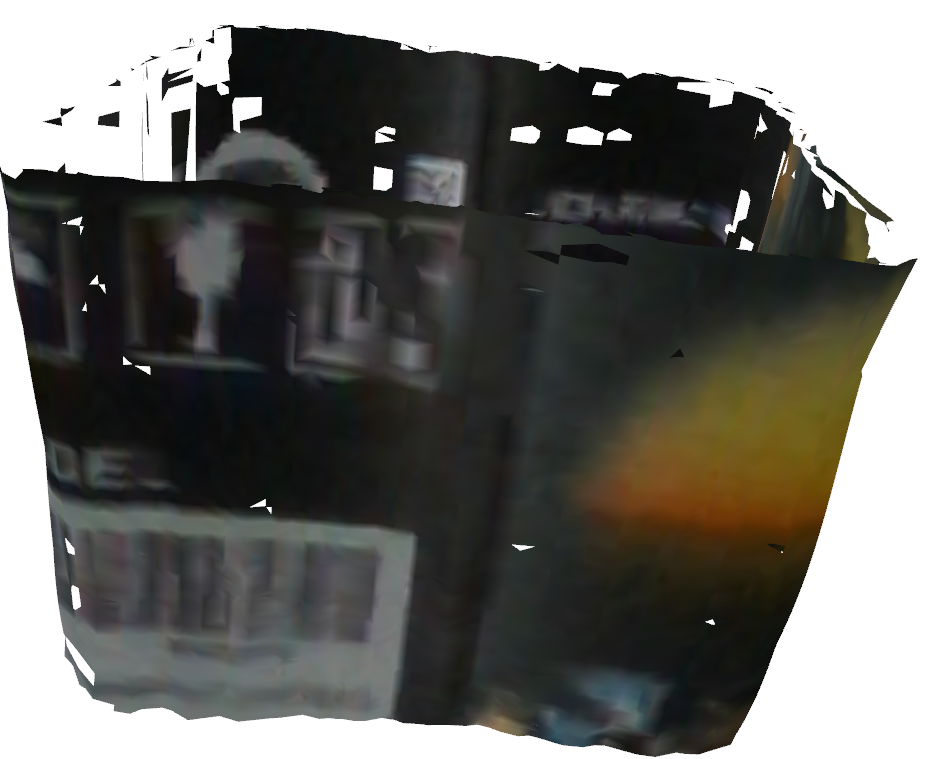
\includegraphics[scale=0.2]{bpaBox7x.PNG}
    \end{minipage}
\caption{Mesh utworzony za pomocą BPA dla jabłka oraz pudełka.}
\label{fig:appleBoxBpa}
\end{figure}

\begin{figure}[H]
  \centering
  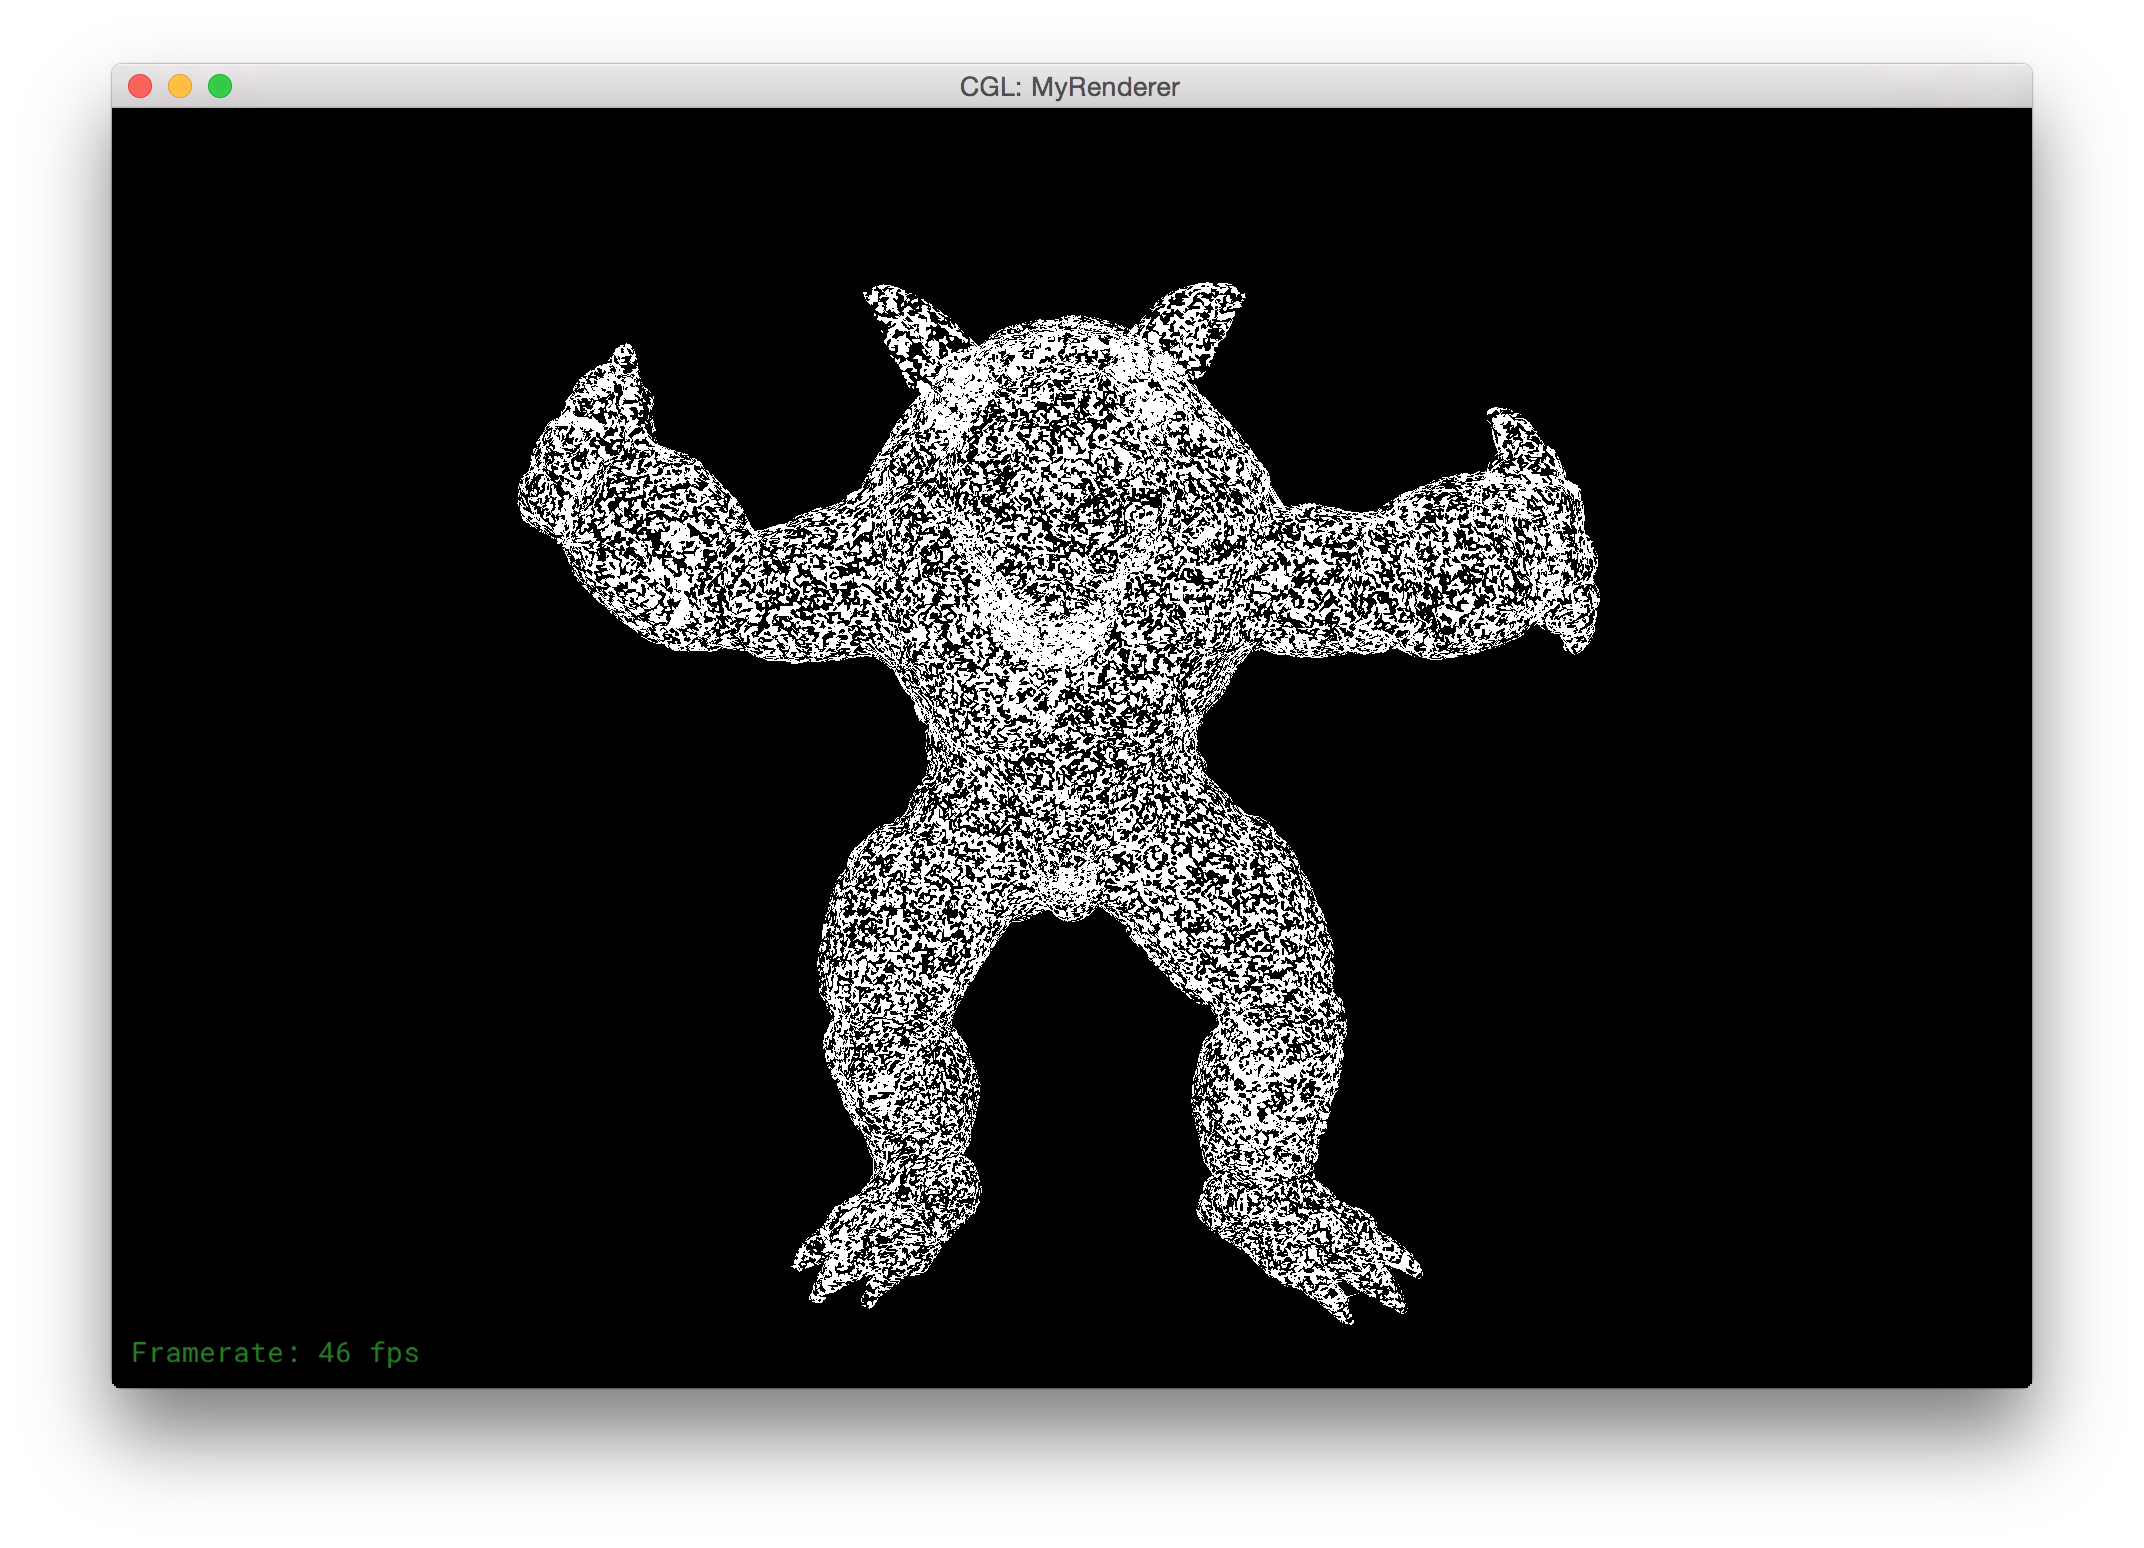
\includegraphics[scale=0.3]{armadilloBpa.png}
  \caption{Mesh człowieka armadillo wygenerowany za pomocą BPA \cite{bpaGit}.}   
  \label{fig:armadillo}
\end{figure}
W meshu człowieka Armadillo można zauważyć wiele luk. Autorzy stwierdzili, że ciężko im było dobrać odpowiedni promień kuli, dla którego powierzchnia obiektu stałaby się gładka. Na danym przykładzie widać, że algorytm BPA ma swoje wady które czasami utrudniają generację poprawnego modelu. Dla autorskich modeli również występują dziury, lecz jest ich o wiele mniej.

Na rysunku \ref{fig:delaAppleBoxComp} oraz \ref{fig:tetGenPicks} zestawione zostały wyniki triangulacji Delaunay'a wykonane za pomocą autorskiego programu oraz przez program TetGen firmy Wias-Berlin.

\begin{figure}[H]
\centering
    \begin{minipage}[b]{0.45\linewidth}
        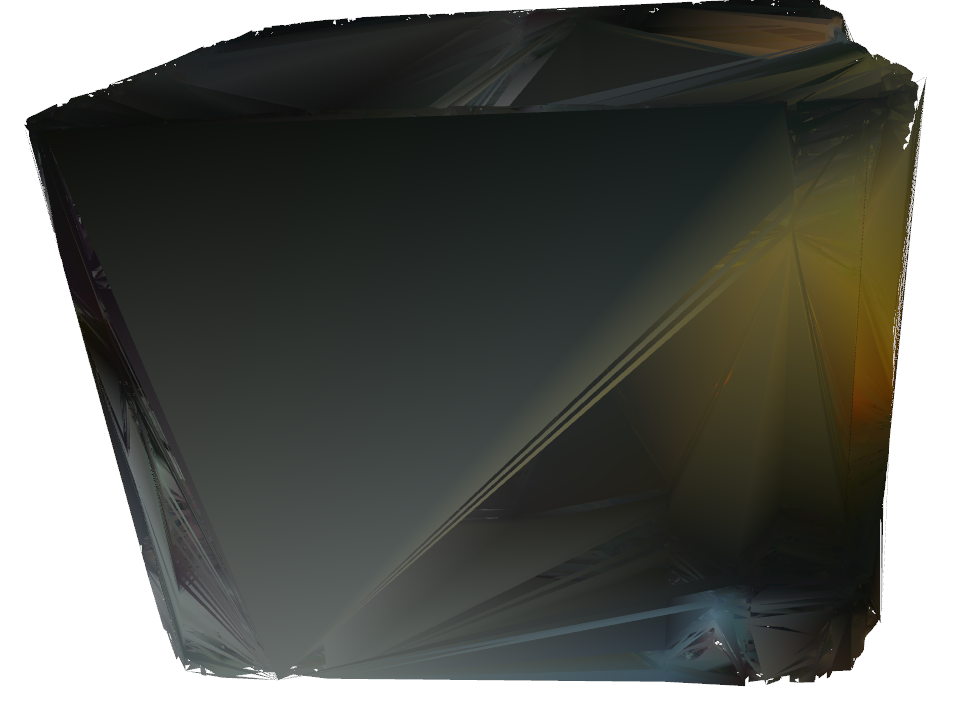
\includegraphics[scale=0.2]{delaunayBox.PNG}
    \end{minipage}
\quad
    \begin{minipage}[b]{0.45\linewidth}
        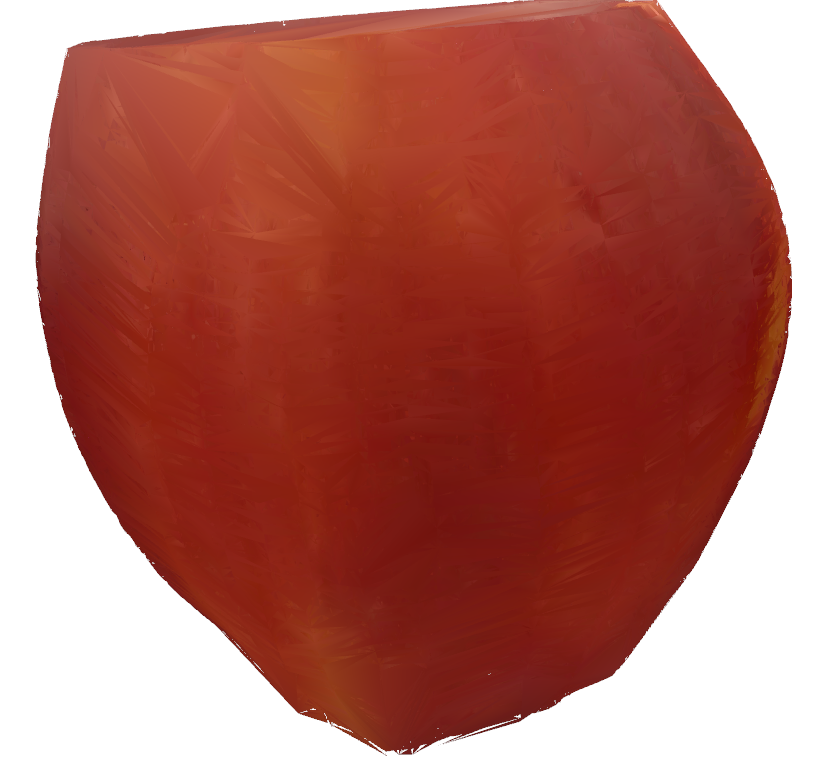
\includegraphics[scale=0.2]{jablkoDelNowe.PNG}
    \end{minipage}
\caption{Mesh utworzony za pomocą triangulacji Delaunay'a dla jabłka oraz pudełka.}
\label{fig:delaAppleBoxComp}
\end{figure}

\begin{figure}[H]
\centering
    \begin{minipage}[b]{0.45\linewidth}
        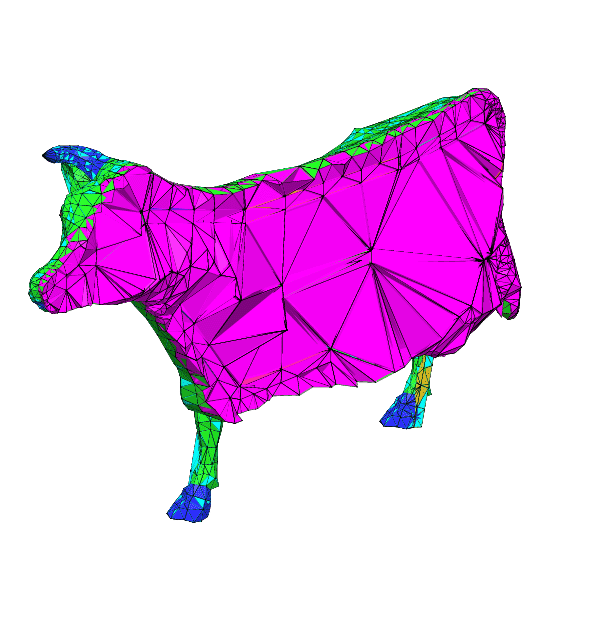
\includegraphics[scale=0.2]{cowDelIg.png}
    \end{minipage}
\quad
    \begin{minipage}[b]{0.45\linewidth}
        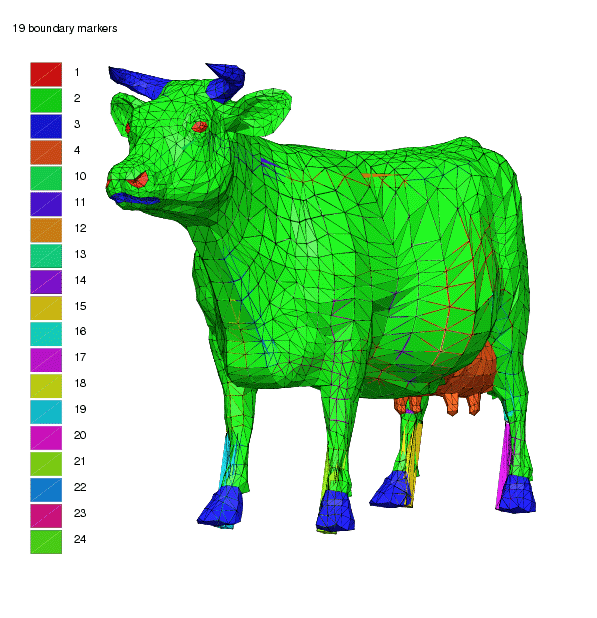
\includegraphics[scale=0.2]{cowPointsImg.png}
    \end{minipage}
\caption{Mesh triangulacji Delaunay'a oraz chmura punktów z przykładowych zdjęć programu TetGen \cite{tetGenWebsite}.}
\label{fig:tetGenPicks}
\end{figure}
Powyżej można zauważyć, że nawet obiekt wygenerowany przez profesjonalne oprogramowanie TetGen zawiera wiele niedoskonałości. Na początkowej chmurze punktów krowy, powierzchnia jest gładka. Jednak po poddaniu obróbce przez triangulację powierzchnia staje się kanciasta i zawiera wiele odstających ścian. Z kolei istotnym elementem jest brak dziur na powierzchni. Poddając modele z programu obróbce w programie Blender, można by się było pozbyć części niedoskonałości powierzchni. Porównując autorskie obiekty oraz te pochodzące z biblioteki programu firmy Wias-Berlin można dostrzec wiele podobieństw. Wynika to z użycia tego samego algorytmu, a różnice wynikają jedynie z innego podejścia do implementacji.


\section{Błędy oraz możliwości poprawy}
Podczas wykonywania testów zaimplementowanych metod napotkano szereg niedoskonałości. Istnieją również możliwości poprawy istniejących rozwiązań. Część z nich wynika z użytych algorytmów i metod, natomiast inne wynikają z ograniczeń sprzętowych. Poniżej przedstawione zostaną rozwiązania, których zaimplementowanie pozwoli na usprawnienie programu. Umożliwią one również zwiększenie jakości otrzymanych modeli obiektów.

Pierwszym mankamentem istniejącej metody skanowania obiektów jest brak możliwości rejestrowania przezroczystych oraz błyszczących obiektów. Wynika to z zasady działania kamery 3D. Rzutuje ona siatkę interpolacyjną na mierzony obiekt. Jednak, gdy jest on przezroczysty lub błyszczący to odbija on promień lasera. Przez dyfrakcję światła, tylko część zostaje odbita do kamery. By temu zapobiec należy użyć sprawić by obiekt odbijał mniej światła w przypadku obiektów błyszczących oraz sprawić by je odbijał w przypadku przezroczystych. By tego dokonać należy na przykład pomalować powierzchnię na matowy kolor lub przykleić taśmę. Jest to skuteczna metoda pozwalająca na akwizycję danych z tego typu obiektów. 

Kolejnym problemem który został napotkany podczas testów jest brak możliwości skanowania skomplikowanych kształtów. Jeżeli obiekt posiada wystające elementy to mogą one nie zostać zeskanowane poprawnie. W przypadku na przykład kubka, jeśli wiązka światła trafi na jego ucho, to nie zeskanuje ona tego co jest pod spodem. W efekcie na uzyskanym obiekcie będzie widać wystający element, lecz nie to co jest pod nim. By temu zapobiec można dokonać kilku skanów, przemieszczając przy tym obiekt wzdłuż tacki. Dzięki temu jego oś obrotu zostanie przesunięta i zostanie on zeskanowany z innej strony. Dzięki temu będzie można zeskanować powierzchnię pod wystającym elementem.

Wykorzystanie metody triangulacji Delaunay'a jest bardzo kosztowne obliczeniowo. Z przeprowadzonych testów wynika, że czas trwania programu wynosi około 10 minut. Pomimo wykonania szeregu optymalizacji algorytm wciąż trwa znacznie dłużej, niż BPA dla małej długości promienia. W celu dalszej optymalizacji należy przekształcić algorytm, by wykonywał obliczenia równoległe na karcie graficznej. Kolejną możliwością jest utworzenie programu w innym języku. Utworzenie metody wykorzystującej dany algorytm w c++ pozwoli na dokonywanie szybszych obliczeń. Ten język charakteryzuje się lepszym wykorzystaniem mocy obliczeniowej procesora oraz wydajniejszym zarządzaniem pamięcią. Aktualnie język cython, pomimo tego, że jest częściowo kompilowany wciąż zawiera szereg ograniczeń wywodzących się z pythona. Poprzez zastosowanie list o nieokreślonej objętości, zarządzanie pamięcią jest mniej efektywne, a czas operacji jest dłuższy. 

Dokładność skanów jest czymś, na czym należałoby się skupić najbardziej. Istnieje wiele możliwości jej udoskonalenia. W celu zwiększenia precyzji można podnieść liczbę klatek na sekundę nagrania. Dzięki czemu zwiększone zostanie zagęszczenie punktów chmurze. Zwiększona gęstość punktów wpłynie pozytywnie na luki w algorytmie BPA. Jednocześnie przy wykorzystaniu triangulacji Delauny'a gęstsze rozmieszczenie punktów w chmurze wpływa na zmniejszenie wielkości ścian generowanych trójkątów. Gdy pola trójkątów interpolacyjnych będą mniejsze, to będą one siebie nawzajem mniej zakrywać. Poprzez taki zabieg, tekstura obiektu zostanie wierniej oddana. Zmniejszając prędkość obrotową tacki można uzyskać ten sam rezultat, co w przypadku zwiększania liczby klatek. Przy wolniejszym ruchu tacki, wykonane zostanie więcej zdjęć. Wydaje się to być lepszym rozwiązaniem, ponieważ prędkość transmisji danych przez protokół USB nie będzie już ograniczeniem, wzrośnie jedynie czas pomiaru. Kolejnym sposobem na zwiększenie dokładności modeli jest ekstrapolacja kolumn. W tym celu należy w puste przestrzenie pomiędzy kolejnymi kolumnami dodać nowe. Dokonanie tego będzie możliwe dzięki wykorzystaniu pozycji wcześniejszych punktów. Uśrednione pozycje dwóch sąsiednich punktów będą stanowić pozycję środkowego. Dana operacja może zostać wykonana wielokrotnie. Zwiększy to zagęszczenie punktów, jednak mogą zaistnieć przekłamania. Pomiędzy kolumnami występują efekty nieuchwytne, które są niemożliwe do wyznaczenia. W miejscu gdzie nie znajduje się żaden punkt mogło na przykład być wgłębienie. Przy ekstrapolacji zostanie ono jednak zastąpione uśrednioną wartością z okolicznych punktów. Najlepszym rozwiązaniem wydaje się być wykonanie dodatkowych skanów. Należy zarejestrować w jakich miejscach nastąpiły przekłamania punktów, a następnie uruchomić ponownie skan. Można również zarejestrować kilka pełnych obrotów tacki. Posiadając kilka ujęć tego samego kąta obrotu, będzie można wybrać tę wartość która nie jest przekłamana. Poprzez taki zabieg będzie można uniknąć aktualnie dokonywanej interpolacji punktów. Znane wówczas będą rzeczywiste pozycje punktów, a modele w ten sposób wygenerowane będą wierniej odwzorowywały rzeczywistość. 

Ostatnim widocznym w testach ograniczeniem aktualnie wykorzystywanej metody skanowania trójwymiarowego jest brak górnej oraz dolnej ściany. Wykonując skan od boku, nie ma możliwości wyznaczenia kształtu górnej ściany oraz dolnej ściany. Pierwszym sposobem uniknięcia tego jest wykonanie skanu z różnych perspektyw, a następnie nałożenie różnych części modelu na siebie w programie Blender. Będzie to jednak bardzo skomplikowane, ponieważ należy dokonać ekstrakcji jedynie potrzebnych płaszczyzn. Innym sposobem jest wykonanie skanu pod kątem. Dzięki takiemu zabiegowi, oprócz ścian bocznych zarejestrowana zostanie też ściana górna. Jednakże  taki zabieg znacząco utrudnia przekształcenia geometryczne. Oprócz już istniejących będzie należało dodać dodatkowe, uwzględniające przesunięcie kamery oraz jej kąt względem obiektu.
\newpage



